\tikzset{every picture/.style={line width=0.75pt}} %set default line width to 0.75pt        

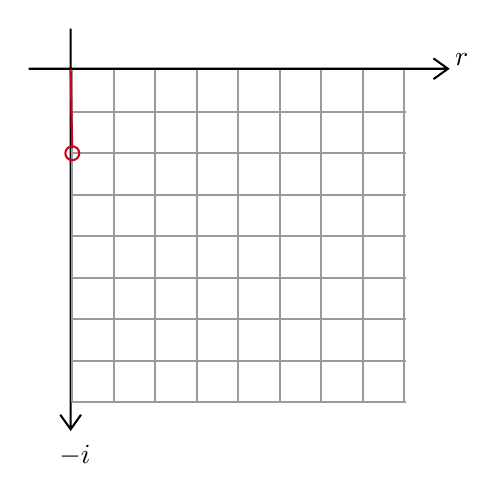
\begin{tikzpicture}[x=0.75pt,y=0.75pt,yscale=-1,xscale=1]
%uncomment if require: \path (0,300); %set diagram left start at 0, and has height of 300

%Shape: Axis 2D [id:dp5907524483347102] 
\draw  (267,55.3) -- (469,55.3)(287.2,229) -- (287.2,36) (462,60.3) -- (469,55.3) -- (462,50.3) (282.2,222) -- (287.2,229) -- (292.2,222)  ;
%Shape: Grid [id:dp6199898397920625] 
\draw  [draw opacity=0] (288,216) -- (449,216) -- (449,56) -- (288,56) -- cycle ; \draw  [color={rgb, 255:red, 155; green, 155; blue, 155 }  ,draw opacity=1 ] (288,216) -- (288,56)(308,216) -- (308,56)(328,216) -- (328,56)(348,216) -- (348,56)(368,216) -- (368,56)(388,216) -- (388,56)(408,216) -- (408,56)(428,216) -- (428,56)(448,216) -- (448,56) ; \draw  [color={rgb, 255:red, 155; green, 155; blue, 155 }  ,draw opacity=1 ] (288,216) -- (449,216)(288,196) -- (449,196)(288,176) -- (449,176)(288,156) -- (449,156)(288,136) -- (449,136)(288,116) -- (449,116)(288,96) -- (449,96)(288,76) -- (449,76) ; \draw  [color={rgb, 255:red, 155; green, 155; blue, 155 }  ,draw opacity=1 ]  ;
%Straight Lines [id:da9323494469903814] 
\draw [color={rgb, 255:red, 208; green, 2; blue, 27 }  ,draw opacity=1 ]   (287.2,55.3) -- (287.95,93.65) ;
\draw [shift={(288,96)}, rotate = 88.87] [color={rgb, 255:red, 208; green, 2; blue, 27 }  ,draw opacity=1 ][line width=0.75]      (0, 0) circle [x radius= 3.35, y radius= 3.35]   ;

% Text Node
\draw (289.23,248) node [anchor=south] [inner sep=0.75pt]    {$-i$};
% Text Node
\draw (471,46.4) node [anchor=north west][inner sep=0.75pt]    {$r$};

\end{tikzpicture}
